\chapter{Introducción}

En este capítulo se ubicará el proyecto en el contexto del robot submarino OpenROV y se enumeraran los distintos problemas que se presentan.
Se expondrá el montaje y puesta a punto del OpenROV y la integración del framework ROS a la arquitectura del robot submarino.
Por último se comentará la estructura de la memoria y se explicarán brevemente las partes por las que está formada.

\section{Robótica móvil}
\label{cap:roboticamovil}
Tradicionalmente las aplicaciones de la robótica estaban centradas en los sectores manufactureros más desarrollados para la producción masiva: industria del automóvil,transformaciones metálicas, etc.

A principios de los años sesenta se introducen en la industria, de modo significativo, los robots manipuladores como un elemento más del proceso productivo.

Los trabajos desarrollados por los robots manipuladores consistían frecuentemente en tareas repetitivas.

Una definición correcta de robot móvil plantea la capacidad de movimiento sobre entornos no estructurados, de los que se posee un conocimiento incierto, mediante la interpretación de la información suministrada a través de sus sensores y del estado actual del vehículo. 

En general se considera que existen tres clases de robots:
\begin{itemize}
\item \textbf{Industriales} son los de mayor difusión en tareas de alcance económico, formados por una estructura mecánica articulada, que se mueve adoptando distintas configuraciones por las órdenes recibidas de un equipo de control basado normalmente en un microprocesador.
\item \textbf{Medicos}  de cooperación o de rehabilitación están concebidos como prótesis inteligentes para los disminuidos físicos. Se procura que tenga la estética correspondiente a la extremidad humana.
\item \textbf{Móviles} son dispositivos de transporte automático, es decir, una plataforma mecánica dotada de un sistema de locomoción capaz de navegar a través de un determinado ambiente de trabajo.

Los robots móviles operando en grandes ambientes no estructurados deben enfrentarse con significativas incertidumbres en la posición e identificación de objetos, la complejidad es tal que, trasladarse desde un punto A hasta un punto B es una actividad arriesgada para un robot móvil.
El principal problema a resolver en un robot móvil es generar trayectorias y guiar su movimiento.

El robot móvil autónomo se caracteriza por una conexión inteligente entre las operaciones de percepción y acción, que define su comportamiento y le permite llegar a la consecución de los objetivos programados sobre entornos con cierta incertidumbre.
  \begin{itemize}
  \item \textbf{Percepción} La capacidad de percepción del robot móvil se traduce en la síntesis de toda la información provista por los sensores, con el objeto de generar mapas globales y locales del entorno de acuerdo a los diversos niveles de control. 
  \item \textbf{Razonamiento (acción)}  El robot móvil debe ser capaz de decidir que acciones son requeridas en cada momento, según el estado del robot y el de su entorno, para alcanzar su(s) objetivo(s).
  \end{itemize}
\end{itemize}


\section{Robots Submarinos}
\label{cap:Robots Submarinos}
Durante los últimos años, el uso de vehículos robots submarinos ha aumentado rápidamente, desde que tal vehículo se puede operar en las áreas más profundas y más arriesgadas que buzos no pueden alcanzar. Entre las aplicaciones potenciales de tales vehículos tenemos el área de la pesca, control submarino de contaminación, y la manipulsación y limpieza del océano, así como de sitios nucleares.

Se trata de un área de diversas aplicaciones en el mundo real, ya que permite y facilita la exploración, la búsqueda y rescate y estudios científicos en zonas muy profundas del mar, a pesar de problemas que se pueden presentar, como son la alta dinámica y la naturaleza del ruido del medio submarino, así como también la carencia de puntos de referencia y las limitaciones en las comunicaciones por efecto del agua.

Podriamos diferenciar las diferentes áreal potenciales en las cuales tienen una aplicación como:

  \begin{itemize}
  \item \textbf{Ciencia}
    \subitem Generación de mapas del suelo marino.
    \subitem Rápida respuesta a eventos eceanográficos y geotérmicos.
    \subitem Muestreo geológico
  \item \textbf{Militar}
   \subitem Búsqueda y eliminación de minas submarinas. 
   \subitem Reconocimiento de rutas, áreas y zonas. 
   \subitem Vigilancia de áreas de interés. 
   \subitem Búsqueda y rescate en combate. 
   \subitem Adquisición de objetos. 
   \subitem Ajuste indirecto de armas de fuego. 
   \subitem Seguridad en zonas cercanas. 
   \subitem Soporte al desarrollo de la situación. 
   \subitem Soporte a la preparación del campo de batalla. 
   \subitem Soporte a la evaluación de daños en batalla.
  \item \textbf{Minería oceánica e industria del petróleo}
    \subitem Estudio del oceano y evaluación de recursos.
    \subitem Construcción y mantenimiento de estructuras submarinas.
  \item \textbf{Otras}
    \subitem Inspección en barcos del casco y los tanques internos.
    \subitem Inspección de plantes nucleares.
    \subitem Instalación e inspección de cables de comunicación y energía. 
    \subitem Paseos turísticos bajo el mar.
    \subitem Etc.
 \end{itemize}

\begin{figure}[hbtp]
  \begin{center}
    \subfigure[Robot Deep Trekker]{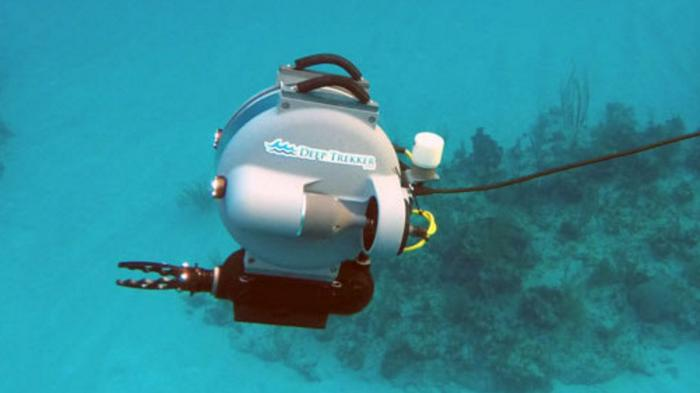
\includegraphics[width=6cm,height=5cm]{img/cap1/submarino1}}
    \subfigure[Robot OpenROV]{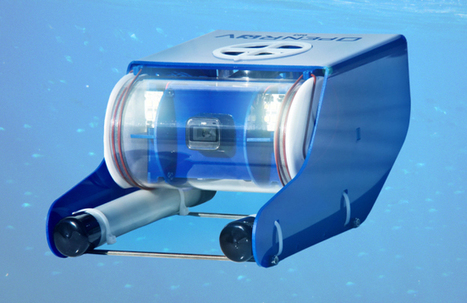
\includegraphics[width=6cm,height=5cm]{img/cap1/submarino2}}
  \end{center}
  \caption{Robots submarinos}
  \label{fig:submarino}
\end{figure}
  
\section{ROS}
\label{cap:ROS}

Sistema Operativo Robótico (en inglés \textit{Robot Operating System, ROS}\footnote{http://wiki.ros.org/}) es un framework para el desarrollo de software para robots que provee la funcionalidad de un sistema operativo en un clúster heterogéneo. 

ROS provee los servicios estándar de un sistema operativo tales como abstracción del hardware, control de dispositivos de bajo nivel, implementación de funcionalidad de uso común, paso de mensajes entre procesos y mantenimiento de paquetes. Está basado en una arquitectura de grafos donde el procesamiento toma lugar en los nodos que pueden recibir, mandar y multiplexar mensajes de sensores, control, estados, planificaciones y actuadores, entre otros.

ROS tiene dos partes básicas: la parte del sistema operativo, ros, como se ha descrito anteriormente y ros-pkg, una suite de paquetes aportados por la contribución de usuarios (organizados en conjuntos llamados pilas o en inglés stacks) que implementan la funcionalidades tales como localización y mapeo simultáneo, planificación, percepción, simulación, etc.

ROS es software libre bajo términos de licencia BSD. Esta licencia permite libertad para uso comercial e investigador. Las contribuciones de los paquetes en ros-pkg están bajo una gran variedad de licencias diferentes.

\section{Estructura de la memoria}
\label{cap:estructuradelamemoria}
En este documento se describen los aspectos más relevantes del desarrollo y montaje del robot. La memoria esta dividida en 6 capítulos. 
El primer capítulo, Introducción, se ha realizado una presentación de los robot móviles, en particular, del robot submarino OpenROV. En el segundo capítulo se define el problema y se establecen los objetivos. El montaje del robot se especifica en el tercer capítulo. En el siguiente capítulo, el cuarto, se explicará el entorno y las herramientas utilizadas. En el quinto capítulo, se mostrará la integración del OpenROV con ROS y en el último, el sexto, habrá ejemplos de como ha funcionado el robot en un entorno real.
